\section*{Exercise 16}
\addcontentsline{toc}{section}{Exercise 16}
For a$2^{128}$ key size we divide the resources according to the recommendation
from the lectures: $2^{l/3}$ where l is the key size. This gives us:\\
\begin{tabular}{c|c|c}
m & $2^{l/3} $&$ 2^{42}$\\
t & $2^{l/3} $&$ 2^{42}$\\
L & $2^{l/3} $&$ 2^{42}$
\end{tabular}\\
Inserting these in the table from the slides gives us the following
computation/memory requrements.\\
\begin{tabular}{l|cc}
\  & Hellman & Rainbow\\\hline
Precomp Encryption 	& $O(2^{128})$ & $O(2^{128})$\\
Precomp. Sorting 	& $O(2^{84})$ & $O(2^{84})$\\
Memory				& $O(2^{84})$ & $O(2^{84})$\\
Online Encryptions	& $O(2^{84})$ & $O(2^{84})$\\
Online Searching	& $O(2^{84})$ & $O(t)$\\
\end{tabular}
\section*{Exercise 17}
\addcontentsline{toc}{section}{Exercise 17}
My understanding of the new funktion to be implemented: $f_i(x) = f(x) \oplus i$ 
is that the program should continue to use the MD5 from Exercise 15 but the
result of that function should be XOR'ed with i, where $i = [0, 2^8]$ is the
current position in the chain. The table is still build with random
non-repeating starting points.\\
to do this my code is simply:
\begin{lstlisting}
	public static int getMD5Hash(int hexInput, int i, int bitSizeLimiter)
	{
		int temp = getMD5Hash(hexInput, bitSizeLimiter);
		temp = temp ^ i;
		return temp;
	}
\end{lstlisting}
where \lstinline{getMD5Hash(int, int)}
is the original function used in Excercise 15.\\
Running the same test with the new function yilds a much better $\approx
98\%$ coverage of the keyspace, it's also easy to see in
figure~\ref{fig:Rainbow} that a high coverage is atained much faster than in
execise 15.
\FloatBarrier
\begin{figure}[h]
\centering
\makebox[\textwidth]{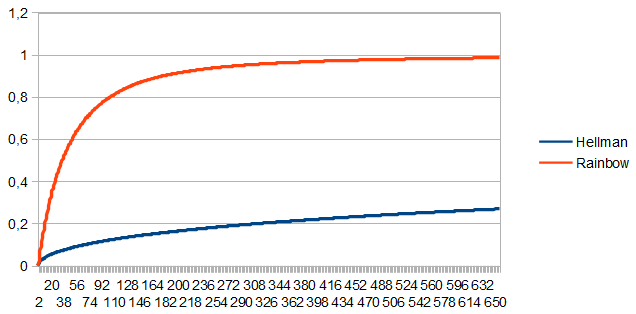
\includegraphics[width=\textwidth]{Rainbow}}
\caption{\emph{Coverage}: The rainbowtable-style vs the simple 
Hellman-like table}
\label{fig:Rainbow}
\end{figure}
\FloatBarrier